\documentclass[11pt,a4paper]{article}
\usepackage[utf8]{inputenc}
\usepackage[T1]{fontenc}
\usepackage[spanish,es-noshorthands]{babel}
\usepackage[margin=2.2cm]{geometry}
\usepackage{amsmath,amssymb}
\usepackage{graphicx}
\usepackage{booktabs}
\usepackage{longtable}
\usepackage{xcolor}
\usepackage{pdflscape}
\usepackage{enumitem}
\usepackage[colorlinks=true,linkcolor=blue!50!black,urlcolor=blue!50!black]{hyperref}
\graphicspath{{../../simulacion/pendulo_invertido/resultados/}}
\setlength{\parskip}{5pt}
\setlength{\parindent}{0pt}

\title{Qué se hizo el 15 de octubre\\[4pt]
\large Péndulo invertido en Simulink, el motor real, y dos errores que encontramos}
\author{Segway con patas -- Robótica II, UNCUYO}
\date{15 de octubre de 2026}

\begin{document}
\maketitle

\noindent\fbox{\parbox{0.97\textwidth}{\textbf{Para Francisco y Matías.} Esto resume una sesión larga
de trabajo sobre el péndulo invertido. Hay cosas que tocan archivos de ustedes, así que conviene
leerlo antes de hacer \texttt{pull}. Al final (sección 7) está lo que le toca a cada uno.}}

\section{Lo que cambió, en cuatro líneas}

\begin{enumerate}[nosep]
\item El modelo tenía cargado un motor que \textbf{no es el que compramos}. Ya está el GA25-370 1:20.
\item El péndulo invertido ahora corre \textbf{en Simulink}, con el motor y el LQR, y hace las dos
  cosas: quedarse parado e ir a otra posición.
\item Encontramos \textbf{dos errores de cálculo} y una conclusión que estaba mal, y los corregimos.
\item Escribimos la \textbf{justificación de por qué usamos LQR}, para la defensa.
\end{enumerate}

Todo está verificado: la suite pasa 24 de 24 pruebas.

\section{El motor: ahora es el que compramos}

El modelo suponía un JGB37-520 con reducción 1:30 y 152 g. Compramos un \textbf{GA25-370 1:20 de
300~rpm}, que es el que Matías documentó en \texttt{ROB-011}. Cambió todo lo que dependía de eso.

\textbf{Pero la ficha del vendedor se contradice a sí misma}, y esto conviene saberlo. La parte
eléctrica cierra bien: resolviendo los puntos de vacío y de carga da $R = 10{,}28~\Omega$, que predice
1,17~A de bloqueo contra los $\le 1{,}1$~A que declara. La columna de torsión, en cambio, es
inservible: su punto de carga exigiría un rendimiento del reductor del 18\,\% y el de bloqueo del
146\,\%, que es imposible. Y 160~g$\cdot$cm figura idéntico para 1:44 y 1:20, lo que delata un copiar
y pegar.

Por eso \textbf{el par del modelo no se lee de la ficha, se calcula}: da unos 3,1~kg$\cdot$cm por
motor al bloqueo, contra los 5,6 que anuncian. Medirlo con un brazo y una balanza es lo primero que
hay que hacer.

\begin{center}\small
\begin{tabular}{lrr}
\toprule
 & Antes (motor supuesto) & Ahora (motor real) \\
\midrule
Reducción & 1:30 & 1:20 \\
Masa de cada motor & 152 g & 95 g \\
Masa del robot & 1120 g & \textbf{1006 g} \\
Velocidad máxima & 0,64 m/s & \textbf{1,01 m/s} \\
Polo inestable & 6,93 1/s & 7,62 1/s \\
\bottomrule
\end{tabular}
\end{center}

Como el motor cuelga de la rueda, el cambio también movió la dinámica de la pata: la normal estática
bajó de 5,49 a 4,93~N y el golpe del escalón se lleva ahora el 27\,\% de la energía en vez del 35\,\%.
Se recompilaron los PDF de \texttt{dinamica}, \texttt{dcl} y \texttt{cinematica}.

\section{Lo nuevo: el péndulo invertido en Simulink}

Está en \texttt{simulacion/pendulo\_invertido/}. Se arranca con
\textbf{\texttt{INICIAR\_PENDULO\_SIMULINK.m}}: ahí se ponen los parámetros, se construye el modelo si
falta, se simula y se compara contra el modelo de MATLAB. No conviene abrir el \texttt{.slx} solo,
porque sin los parámetros en el workspace no corre.

\begin{center}
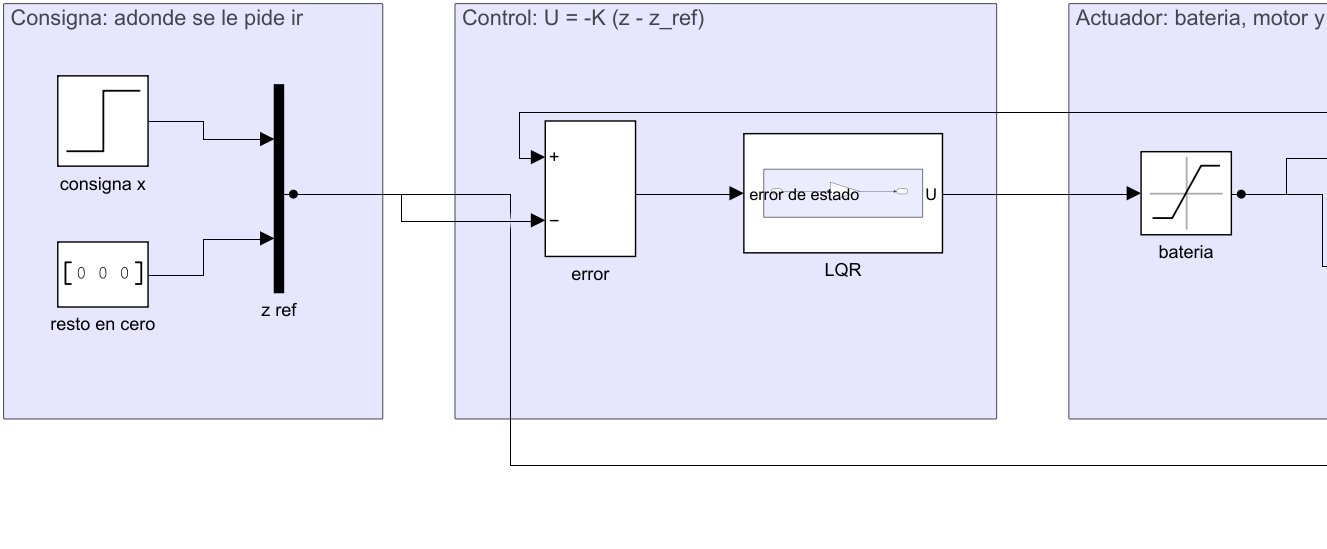
\includegraphics[width=\textwidth]{diagrama_superior_1.png}
\par\vspace{10pt}
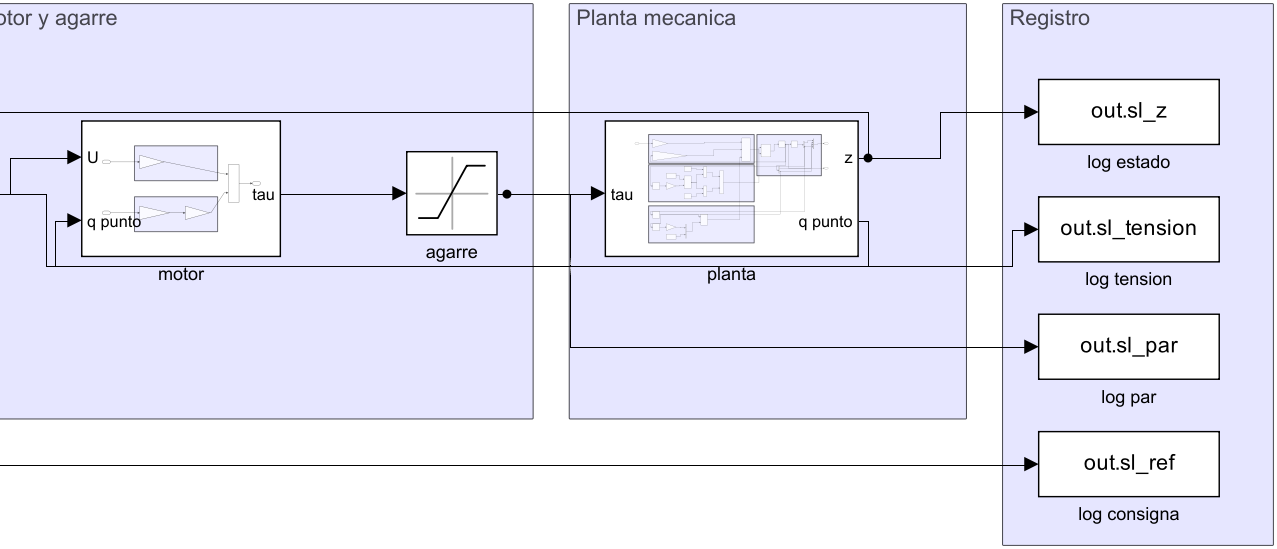
\includegraphics[width=\textwidth]{diagrama_superior_2.png}
\par\vspace{4pt}\small El nivel superior, partido en dos para que se lea: 
arriba la consigna y el control, abajo el actuador, la planta y el registro.
\end{center}

Cinco áreas, que son las cinco etapas físicas: la consigna de adónde ir, el control, los dos límites
del actuador (batería y agarre), la planta y el registro.

\textbf{Sólo bloques nativos}, ni un MATLAB Function: hay una prueba que lo verifica. La planta va en
forma matricial,
\[
M(\varphi)\,\ddot q = H\tau - D\dot q + \sin\varphi\begin{bmatrix}-h\,\omega^2\\ k\end{bmatrix},
\qquad q = \begin{bmatrix}x\\\varphi\end{bmatrix},
\]
con la matriz armada por filas y \textbf{un solo bloque \texttt{Divide} matricial} que resuelve
$M\backslash\text{rhs}$. Dos integradores vectoriales llevan $\ddot q$ hasta $q$. El modelo se genera
desde código (\texttt{construir\_pendulo\_simulink.m}), así que si hay que cambiar la topología se
cambia ahí y se regenera; editar el \texttt{.slx} a mano deja los dos desincronizados.

\textbf{Detalle de nombres:} la tensión se llama \texttt{U} y la velocidad de avance \texttt{v}. Antes
las dos eran \texttt{V} y se confundían.

\subsection*{Qué hace}

\begin{landscape}
\vspace*{\fill}
\begin{center}
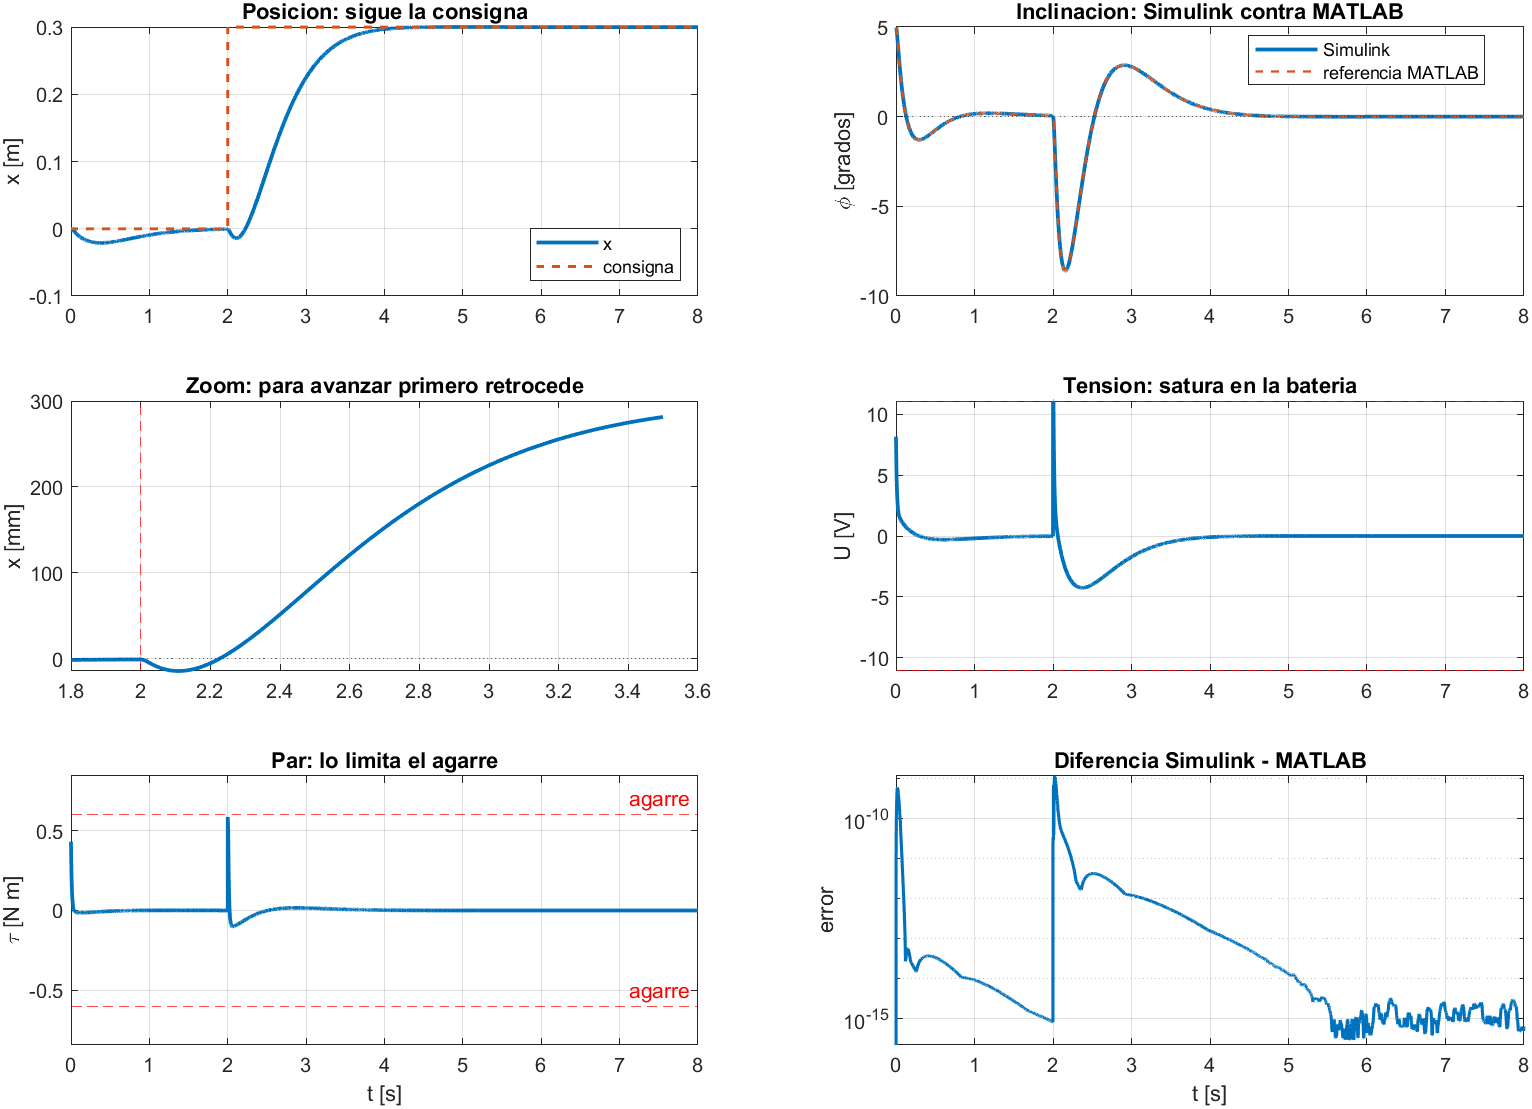
\includegraphics[width=\linewidth]{respuesta_lqr.png}
\par\vspace{6pt}\small Arranca inclinado 5 grados y a los 2 s se le pide ir a 30 cm.
\end{center}
\vspace*{\fill}
\end{landscape}

Arranca inclinado 5$^\circ$, se endereza corriéndose 21~mm, y a los 2~s se le pide ir a 30~cm: llega
con error nulo en 1,83~s. Coincide con el modelo de MATLAB a $2\cdot10^{-12}$.

Mirá el panel de abajo a la izquierda: \textbf{para avanzar, primero retrocede 13,5~mm}. No es un
error del control, es el cero en el semiplano derecho. Las ruedas tienen que salirse de abajo del
centro de masa para que el cuerpo caiga hacia adelante.

\section{Dos errores que encontramos, y una conclusión que estaba mal}

Sometimos todo a una revisión adversaria (38 agentes en paralelo, con refutación independiente de cada
hallazgo). Encontró dos errores reales en el código nuevo.

\subsection*{La fuerza en el piso estaba mal calculada}

Se calculaba como $-\tau_{ef}/r - J_w\ddot x/r^2$, que omite la inercia reflejada del rotor. Con el
reductor 1:20 el error llegaba al 200\,\%, y en caída libre daba el signo contrario. Ahora usa la forma
exacta de Newton sobre todo el robot,
\[
F = m_{tot}\ddot x - h\cos\varphi\,\ddot\varphi + h\sin\varphi\,\dot\varphi^2,
\]
que no se vuelve a romper al agregar inercias. El balance horizontal de la verificación pasó de
$5{,}6\cdot10^{-17}$ a cero exacto.

\subsection*{Y de ahí salía una conclusión falsa}

Habíamos dicho que \emph{``el motor puede empujar varias veces más de lo que el piso aguanta, así que
el actuador que limita es el neumático''}. \textbf{Es falso.} La cuenta usaba $\tau/r$, que no es la
fuerza en el contacto porque parte del par acelera el rotor (0,44~kg reflejados sobre un robot de
1,0~kg).

\begin{center}\small
\begin{tabular}{lr}
\toprule
$\tau/r$ (lo que usábamos) & 17,8 N \\
\textbf{Fuerza real en el piso} & \textbf{6,0 N} \\
Fricción disponible ($\mu = 0{,}7$) & 6,9 N \\
\bottomrule
\end{tabular}
\end{center}

O sea que el motor usa el \textbf{87\,\% del agarre} y no llega a hacer patinar la rueda. Están casi
empatados: con $\mu = 0{,}6$ el motor ya pasaría a ser el limitante.

\subsection*{Y el diseño del LQR no sobrevivía a la implementación}

Este es el hallazgo más serio. El LQR con la regla de Bryson pura ponía un polo en $-189$~1/s que no
tiene nada que ver con la física del robot (el más rápido de la planta es $-7{,}6$): era puro costo de
implementación. Al agregar lo que el robot real va a tener --- muestreo de 5~ms, retardo de cómputo y
el filtro que la cuantización del encoder obliga a poner --- el lazo quedaba \textbf{inestable}.

\begin{center}\small
\begin{tabular}{lccc}
\toprule
 & Polo caro & Margen de muestreo & Con filtro de 20 Hz \\
\midrule
Bryson puro & $-189$ & 1,2$\times$ & \textbf{INESTABLE} \\
\textbf{Bryson $\times$ 4} & $-98$ & \textbf{2,6$\times$} & estable \\
\bottomrule
\end{tabular}
\end{center}

Se corrigió multiplicando $R$ por 4, que cuesta un 8\,\% de tiempo de respuesta. Hay una prueba nueva
que lo verifica para que no vuelva a pasar.

\section{Por qué LQR}

Está desarrollado en \texttt{docs/gestion/2026-10-15-justificacion-lqr.md}. El resumen:

\textbf{No hay evidencia de que la cátedra lo pida} --- en \texttt{guias\_catedra/} sólo hay dos
procedimientos de preselección que no mencionan control --- así que la elección la tenemos que
defender entera.

El argumento que resiste es: la física obliga a realimentar los cuatro estados (con el ángulo solo el
lazo es inestable por estructura; agregando velocidad se sostiene pero la posición queda libre), y una
vez que hay que elegir cuatro ganancias de una sola vez, el LQR es el método que las calcula y el
único que trae una garantía demostrable. \textbf{Lo que no hay que decir} es que el LQR sea mejor que
un PID: verificamos que la $K$ del LQR \emph{es exactamente} una cascada de PD de ángulo más PD de
posición. Son la misma ley escrita distinto.

\section{Estado del repositorio}

\textbf{Nada está commiteado todavía}, y hay algo importante antes de hacerlo (sección 7).

\begin{center}\small
\begin{tabular}{ll}
\toprule
Archivos nuevos & 6 en \texttt{modelado/planta/pendulo\_invertido/} y \texttt{simulacion/} \\
Archivos modificados & 24 \\
Pruebas & \textbf{24 de 24} \\
\bottomrule
\end{tabular}
\end{center}

Para correr todo, desde la raíz:
\begin{verbatim}
  runtests('modelado/dinamica/tests')
  runtests('simulacion/pendulo_invertido/tests')
  runtests('simulacion/dinamica_pata_v1/tests')
\end{verbatim}

\section{Lo que le toca a cada uno}

\subsection*{Para Francisco (el CAD)}

\begin{enumerate}[nosep]
\item \textbf{La tapa de 114 g no existe} en el ensamble de la segunda iteración, y el modelo la está
  contando. Hay que agregarla al CAD o sacarla del modelo.
\item Tu \texttt{mass\_properties.md} de SolidWorks da \textbf{587,7 g de ensamble contra los 802 g}
  que el modelo estima por volumen. Una diferencia del 36\,\% que nadie reconcilió. Esa salida tuya
  es el dato más confiable que tenemos y hoy el modelo la ignora.
\item Faltan la rueda y el motor en el ensamble de la segunda iteración, así que no se puede cerrar la
  ficha de masas.
\item El CAD todavía tiene el motor viejo (37~mm) y no el GA25-370 (cuerpo 25~mm, caja 21~mm).
\item Sigue pendiente lo de los 3~mm de la bancada en \texttt{cabeza\_v31}.
\end{enumerate}

\subsection*{Para Matías (parámetros y simulación)}

\begin{enumerate}[nosep]
\item Toqué \texttt{parametros\_fisicos.m}: el motor (sección 1 y 7), más dos campos nuevos
  (\texttt{i\_vacio} y \texttt{eta\_reductor}). La variante \texttt{segunda\_iteracion} sigue siendo
  la de por defecto.
\item Generalicé \texttt{ecuaciones\_pendulo\_invertido.m} y
  \texttt{linealizar\_pendulo\_invertido.m} con un campo \texttt{e\_acople} que vale cero por defecto,
  así que \textbf{tu verificación sigue dando 6/6 sin cambios}. Era necesario porque el acople del
  rotor es constante y no cabía dentro de $h$.
\item Tu ficha \texttt{ROB-011} dice que falta la resolución del encoder. La usé como 11~PPR para
  calcular el ruido de cuantización, así que \textbf{ese número hay que confirmarlo contando pulsos}.
\item Los resultados guardados de \texttt{dinamica\_pata\_v1} son de la variante vieja; habría que
  regenerarlos.
\end{enumerate}

\subsection*{Lo más urgente, para cualquiera}

\begin{enumerate}[nosep]
\item \textbf{Pesar todo.} Las masas son estimaciones por volumen.
\item \textbf{Medir el par real del motor} con un brazo y una balanza, y el \textbf{$\mu$ del
  neumático} sobre el piso real: el motor y el agarre están al 87\,\% uno del otro, así que
  cualquiera de los dos puede pasar a limitar.
\item \textbf{Calcular el acoplamiento entre mover las patas y el equilibrio.} Es el agujero más
  grande: el agache de 0,6~s es 1,6 veces más rápido que el asentamiento del LQR, y durante el agache
  la normal cae al 35\,\% del peso. El par de reacción del servo sobre el chasis no está calculado en
  ningún archivo.
\end{enumerate}

\section{Antes de hacer pull o push}

\textbf{La rama local está un commit atrás de \texttt{origin}}: falta el commit de Matías con los
datasheets de electrónica. Y hay cosas que se pisan, así que conviene no hacerlo con GitHub Desktop a
ciegas, que es lo que en septiembre dejó un conflicto commiteado adentro de un archivo.

\begin{enumerate}[nosep]
\item \texttt{BACKLOG.md} lo editamos los dos: va a dar conflicto y hay que resolverlo a mano
  conservando las filas de ambos.
\item Ya corregimos una colisión de identificadores: nuestras filas nuevas pasaron a
  \texttt{ELE-014}, \texttt{ELE-015}, \texttt{ELE-016} y \texttt{DOC-108}.
\item \texttt{README.md} también lo tocamos los dos.
\end{enumerate}

El orden sugerido es: commitear lo nuestro primero, después traer lo de Matías, y resolver el
\texttt{BACKLOG} con las dos partes.

\end{document}
